\problemname{Drebėjimas kasyklose}
\illustration{.4}{img/Goodluck_Mine.jpg}{%
  \emph{Goodluck Mine, Passage} by Ashley Dace. 
  License CC BY-SA 2.0.}

\noindent
Apleistose Moravijos Nykštukų kasyklose įrengtos nedidukės autonominės alaus daryklos
išties yra Nykštukų inžinerijos išradingumo ir meistriškumo įrodymas!
Deja, kartais žemės drebėjimai niokoja kasyklas, vamzdžiai išsiklibina ir iš piltuvų vertingasis skystis pilamas ant grindų.
Jeigu įvyktų žemės drebėjimas, jūs, kaip aukščiausiasis alaus daryklų apsaugos pareigūnas, turite išjungti mašinas visose kasyklų salėse.


Kol tuneliais pasieksite visas mašinas, užtruksite.
Nežiūrint to, norisi, kad visas išlaistyto skysčio kiekis būtų kuo mažesnis.

\medskip
Nykštukų kasyklas sudaro  $n$~salių ir jas jungia $n-1$~tunelis.
Kasyklų sistema yra jungi, tad iš bet kurios salės įmanoma pasiekti bet kurią kitą.
Pereiti tunelį užtrunka $1$~laiko vienetą.
Mašinos išjungimas ir salės perėjimas neužtrunka laiko.
Jei kurioje nors salėje mašina išjungiama praėjus $t$ laiko po žemės drebėjimo, tai mašina jau bus spėjusi išlieti
$t$~litrų skysčio.
Įvyksta lygiai vienas žemės drebėjimas, kuris paveikia visas sales tuo pat metu. 
Be to, jokia mašina negali būti išjungta prieš drebėjimą. 
Pradėti galite bet kurioje iš salių.

\section*{Pavyzdys}

Pirmajame pavyzdyje aprašytos kasyklos atrodo štai taip:

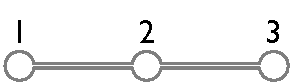
\includegraphics[width=.2\textwidth]{img/sample-1.pdf}

Jeigu pradėtumėte $2$-ojoje salėje ir sales aplankytumėte tvarka $2$, $1$, $2$, $3$, 
tuomet mašinas išjungtumėte laiko momentais~$0$ ($2$-ojoje salėje), ~$1$ ($1$-ojoje salėje) ir~$3$ ($3$-iojoje salėje).
Iš viso būtų išlaistyta $0+1+3=4$~litrų skysčio.
Tačiau jeigu pradėtumėte $1$-ojoje salėje ir sales aplankytumėte tvarka $1$, $2$, $3$, 
iš viso būtų išlaistyti $0+1+2=3$~litrai skysčio, kas yra geriau.

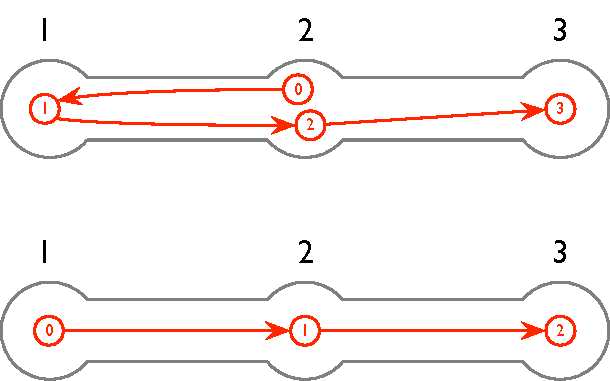
\includegraphics[width=.4\textwidth]{img/sample-1-ans.pdf}

\section*{Pradiniai duomenys}

Pirmoje eilutėje pateiktas salių skaičius $n$ (sveikasis skaičius).
Salės numeruojamos $1$, $\ldots$, $n$.
Kitose $n-1$ eilučių pateikiama po du sveikuosius skaičius $u$ ir $v$, kuriems galioja
$1\leq u < v \leq n$ % constraint:hallnames
ir kurie žymi, kad sales~$u$ ir $v$ jungia tunelis.

\section*{Rezultatai}

Išveskite vieną sveikąjį skaičių: kiek mažiausiai skysčio išsilaistys (litrais).

\section*{Ribojimai ir vertinimas}

Visada galios
$1\leq n\leq 10^5$. % constraint:n

Sprendimas bus testuojamas su keliomis testų grupėmis, kurių kiekviena verta tam tikro skaičiaus taškų.
Kiekviena testų grupė sudaryta iš įvairių testų.
Testų grupės taškai skiriami tik išsprendus visus grupės testus.
Galutinis taškų, skiriamų už šį uždavinį, skaičius, lygus daugiausiai surinkusio sprendimo taškų skaičiui.

\medskip
\begin{tabular}{lll}
Grupė & Taškai & Papildomi ribojimai \\\hline
  $1$ & $18$ & jokia salė neturi daugiau nei dviejų tunelių\\
  $2$ & $19$ & daugiausiai viena salė turi daugiau nei du tunelius\\
  $3$ & $20$ & $n\leq 10$\\
  $4$ & $21$ & $n\leq 1000$\\
  $5$ & $22$ & \emph{nėra}
\end{tabular}
